
\chapter{Particle velocimetry of vortices in Bose–Einstein condensates}\label{chap:velocimetry}

\lettrine[lines=3]{T}{his chapter comprises a feasibility} study for an imaging method for the real time tracking of quantum vortices in a turbulent $^{41}$K condensate. The method involves ultracold $^{87}$Rb tracer particles that become bound to vortex lines in the condensate and are imaged continuously to track the vortex lines as they move. The imaging of tracer particles to track vortex motion has previously proved successful in superfluid helium~\cite{bewley_generation_2009, bewley_superfluid_2006, packard_vortex_1982}, and the method of laser cooling and imaging atoms in high resolution with the same laser light has also been successful in cold atom systems~\cite{bakr_quantum_2009}. This chapter comprises numerical simulations of the method under a number of assumptions to establish its feasibility as an imaging method. 

\begin{figure}
\begin{center}
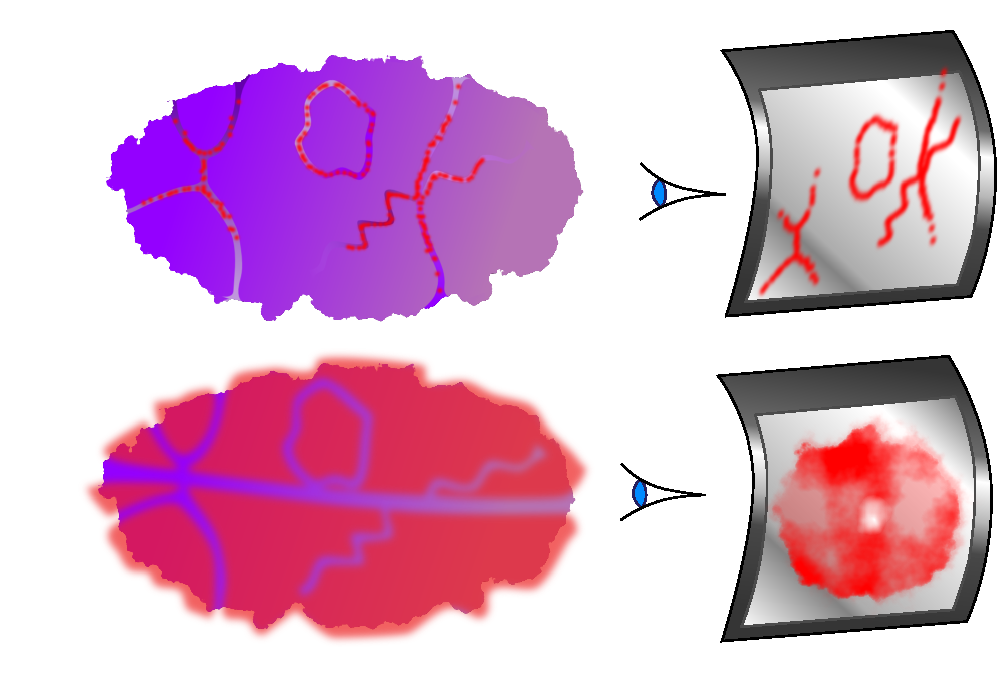
\includegraphics[width=0.6\textwidth]{figures/unsorted/side-on.pdf}
\caption{\label{fig:side-on}Fluorescence imaging of the condensate itself (bottom) makes it difficult to resolve vortices unless they are viewed end-on. The vortex cores are usually smaller than the imaging light's wavelength, and are thus also difficult to resolve unless the cloud is allowed to expand. Imaging tracer particles instead has the potential to resolve both these problems.}
\end{center}
\end{figure}

This method has the potential to overcome several existing difficulties that typical imaging methods face when used to image vortices. In ordinary absorption imaging, atoms are imaged via resonant absorption of the condensate itself, and vortices---visible as density minima---generally can only be seen when the vortex line is normal to the image plane. If not viewed end-on in this way, a vortex line represents only a minor decrease in column density and cannot be distinguished from the rest of the condensate. One solution to this problem is to slice the condensate into layers, and image them separately~\cite{anderson_watching_2001}.

The use of tracer particles that are only present within vortex cores allows vortex lines to be visible from any viewing angle.  Furthermore, since the atoms being imaged reside in the vortex cores themselves rather than the bulk of the condensate, this imaging can potentially be repeatedly or continuously performed without destroying the condensate. This may enable observation of the time evolution of Kelvin waves~\cite{bretin_quadrupole_2003}, vortex reconnections~\cite{leadbeater_sound_2001}, and vortex rings~\cite{anderson_watching_2001}.

This \emph{in-situ} imaging of vortex dynamics may allow more types of vortex motion to be imaged. Dynamics of \bec s are typically studied using a shot-by-shot method, in which repeated experiments with identical initial conditions are imaged destructively after being allowed to evolve for different amounts of time. Whilst this works for many types of dynamics, it fails for experiments that are more sensitive to initial conditions and noise (quantum or otherwise), such as turbulent flow. This includes phenomena which cannot be created reliably in the same initial state, even though the evolution thereafter would be consistent from one experimental run to the next. One such phenomenon is the spontaneous generation of vortices after evaporative cooling~\cite{weiler_spontaneous_2008}.

\emph{In-situ} imaging of vortex motion has been achieved previously \cite{freilich_real-time_2010}, by ejecting a fraction of the atoms from the condensate periodically and imaging them. This process is limited by depletion of the condensate, and was also used only to image vortices end-on. The fraction of the condensate being imaged was also allowed to freely expand before being imaged, since vortex cores are otherwise unable to be resolved by the wavelength of light used. Our method requires neither free expansion or depletion of the condensate.

\section{Motivation: Turbulence}

It is commonly said that turbulence is one of the greatest unsolved problems of classical physics. But in what sense is it an unsolved problem? Its not a problem at all if your aim is reductionism---the Navier--Stokes equation adequately describes the evolution of a Newtonian fluid within its domain of validity, and the process of deriving it from the underlying motion of classical particles is well understood. It's turtles all the way down~\cite[p 1]{hawking_brief_1988}; what more could we ask for?

An demonstrative comparison might be with the field of thermodynamics, as precisely the same statement can be made about the energy content and exchange between systems of particles. Thermodynamics has revealed that despite the chaotic motion of individual particles in an ensemble, definite statements can still be made about the behaviour of the system as a whole, \emph{without having to consider the dynamics of the constituent components in detail}.

This is the kind of solution people have in mind when they speak of `solving' the problem of turbulence. Laws describing the average properties of a fluid without reference to its precise flow field would not simply be interesting as describing turbulence as an emergent phenomenon, but would aid practical computations, which for many problems of interest are prohibitively computationally intensive. The flow of a turbulent fluid contains detail on such a  wide range of length scales that any finite-element or finite-difference analysis of a system such as an aeroplane wing requires a very high resolution in order to be accurate. Following an estimate of computing power required to simulate a turbulent system down to its smallest length scales, Stanley Corrsin quipped~\cite{corrsin_turbulent_1961}:
\begin{quote}
The foregoing estimate  is enough to suggest the use of analog instead of digital  computation; in particular, how about an analog consisting of a tank of water?
\end{quote}
This sounds like a joke, but the reliance of the aerospace industry on wind tunnels and practical tests show that there is some truth to the necessity of using nature as ones computer when it comes to turbulence. Whilst nature must always have the final say, it would be of great benefit to be able to compute expected results more cheaply before setting up a wind-tunnel experiment or constructing a prototype aircraft.

But are we asking for too much? Perhaps the statistical properties of a turbulent fluid fundamentally cannot be decoupled from the finer details. There is reason to believe that this is not the case. There are several tantalising results that hint at universal properties that all turbulent flows share, and there is the simple empirical observation that the average flow of turbulent fluids at large scales is reproducible from one experimental run to the next~\cite[pp 13, 86]{davidson_turbulence:_2004}.

One of these universal results is Kolmogorov's theory of the statistics of small eddies~\cite{kolmogorov_local_1941, spalding_kolmogorovs_1991}. Another is the fact that the rate of energy dissipation via the action of viscosity at small scales is independent of the viscosity itself~\cite[p 77]{davidson_turbulence:_2004}.

Then there is the Richardson energy cascade~\cite{richardson_weather_2007}, in which energy is continually transferred from larger scales to smaller scales. With dissipation at the smallest scales and addition at larger scales, this allows for the existence of `steady state' turbulence.

The above examples derive from ordinary, viscous fluids. Bose--Einstein condensates on the other hand are superfluids. There are several interesting aspects of superfluid turbulence that differ from classical turbulence. The defining difference is the absence of viscosity; another major difference is the quantisation of circulation. On scales much larger than spacing between vortex lines, superfluid turbulence is expected to closely resemble classical turbulence\footnote{Similarly at sufficiently large scales in non-superfluids, velocity gradients are small and hence viscosity can be neglected.}~\cite{tsubota_energy_2009}. But at smaller scales the energy dissipation mechanism is different, instead involving the production of sound waves via vortex interactions~\cite{tsubota_energy_2009, vinen_how_2005}.

In certain 2\textsc{d} geometries, an \emph{inverse cascade}~\cite{onsager_statistical_1949, kraichnan_inertial_1967} is predicted to take place in superfluids, whereby energy moves not from large scales to small, but from small to large, clustering quantised vortices of the same circulation direction together. This phenomenon has been studied numerically in the Monash Quantum Fluids group [CITE] and recently experimentally observed in the Monash Dual-Species lab in experiments performed by Shaun Johnstone, as well as at [OTHER GROUP] [CITE THEM BOTH - ARXIV OR PUBLISHED IF DONE BY THEN]

The following definition of turbulence, taken from~\cite[p 53]{davidson_turbulence:_2004}, emphasises the role of vortices in turbulence in general:
\begin{quote}
Incompressible hydrodynamic turbulence is a spatially complex distribution of vorticity which advects itself in a chaotic manner in accordance with [the vorticity equation\footnote{Which is a transformation of the Navier--Stokes equation for an incompressible fluid into a form in which the vorticity field is center-stage.}]. The vorticity field is random in both space and time, and exhibits a wide and continuous distribution of length and time scales.
\end{quote}

When vorticity exists only in infinitely narrow lines, as it does in superfluid, the vorticity equation mentioned in the above definition reduces to a Biot--Savart type law which can be used to compute the motion of vortices without having to compute the entire flow field.

This is why we are interested in the study of the dynamics of quantised vortices. Unlike in classical fluids, the vortices in superfluids have a definite position and size; there is either a vortex at a given spatial location or there is not. This may make it simpler to describe the motion of vortices statistically.

So far experimental studies of superfluid turbulence have been primarily in the context of liquid helium~\cite{leggett_superfluidity_1999}. Bose--Einstein condensates offer a compelling alternative subject of study for superfluid turbulence. The high degree of control afforded over systems of cold atoms allows the superfluid's properties to be tweaked in several ways, creating a larger parameter space in which to study turbulence than that afforded by liquid helium.

\section{Overview}

[SCRAP THE BELOW: JUST SUMMARISE THE SECTIONS COMING]

Ok, so - the vortices are potential wells. Show some pictures of this.

BUT. PROBLEM. The wells are not very deep when measured in recoil energies. Need cooling! Honours thesis studied this. Answer: maybe.

Possible solution: Feshbach resonance. BUT: problem, cooling doesn't work. To this end, developed a cooling scheme.

Other alternative: sympathetic cooling. We did this too. It looks ok.

Finally: thought about other cooling schemes. Though we didn't simulate this one or take it anywhere, the inability to simulate it prompted me to begin thinking about the issues that the hidden variables chapter resolves.

\begin{itemize}
\item Semiclassical simulations:
Provide details of how the simulations were performed and the results they gave. Describe method of computing collisions between the classically modelled particles and the condensate, and how the fluorescence imaging was simulated. Present results and discuss experimental feasibility.

\item{Sisyphus cooling in a magnetic field}
Describe the scheme for Sisyphus cooling I developed, and show 1D simulation results.

\end{itemize}


\section{Overview of velocimetry scheme}

\begin{figure}
\begin{center}
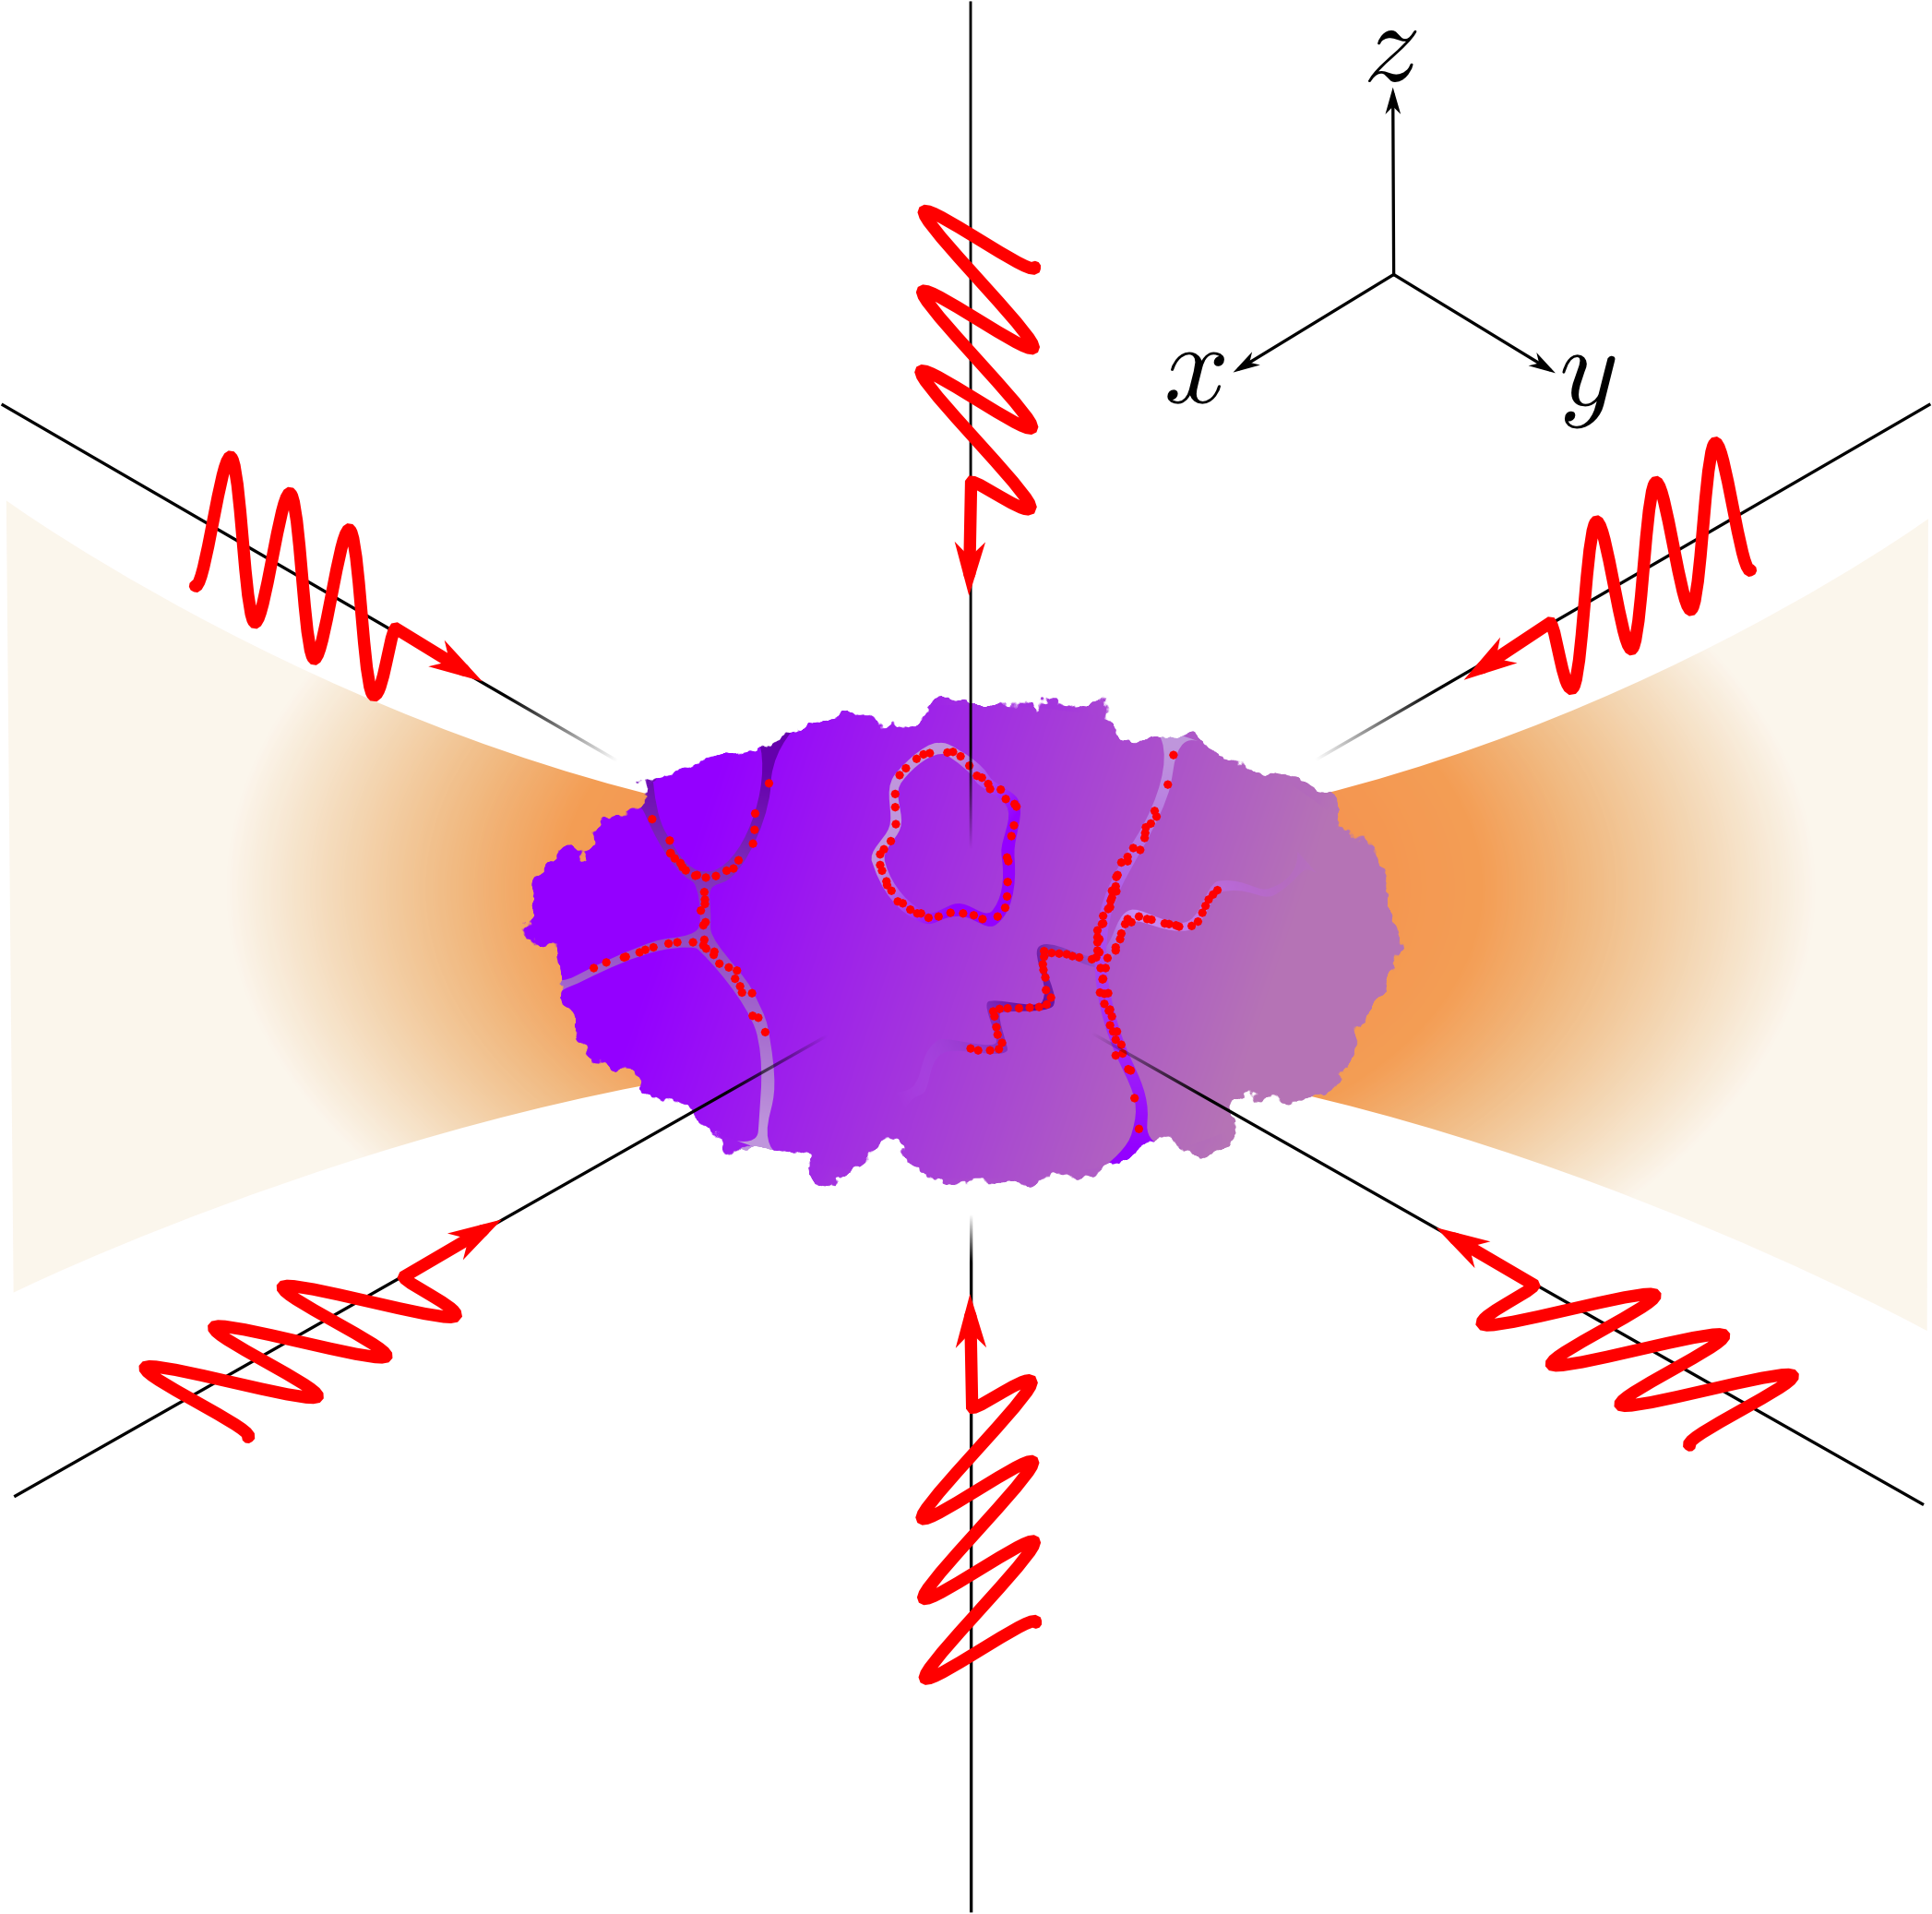
\includegraphics[width=0.6\textwidth]{figures/unsorted/setup.png}
\caption{\label{fig:setup}The simplest scheme for cooling and imaging the tracer particles with the same light is polarisation gradient cooling, involving six slightly off resonant beams (red), with each counterpropagating pair having opposite linear polarisations. This will scatter some light off the tracer atoms, as well as cool them to sub-Doppler temperatures. If the cooling is sufficient, it should encourage the atoms into the vortex cores where their energy is lower, if they aren't already there. Both the rubidium tracers and the potassium \bec\ will be trapped with approximately the same trapping potential by a strong, far off-resonant laser (orange), via the dipole force. Magnetic trapping cannot be used, as polarisation gradient cooling does not work in the presence of a magnetic field.}
\end{center}
\end{figure}

As mentioned, the idea of this method is to use tracer particles to track vortex cores in a \bec\ in real time. The tracer particles are $^{87}$Rb atoms and the BEC made of $^{41}$K. This choice is due to the strong interspecies repulsion between these atoms, which gives rise to the trapping of atoms in the vortex cores. In the limit of low densities and temperatures, such that three body collisions are suppressed and $s$-wave scattering dominates the interspecies interactions \cite[p 120]{leggett_quantum_2006}, the rubidium tracer atoms experience a potential due to the potassium:

\begin{equation}
V(\vec{r}) = \frac{2\pi\hbar^2 a_s}{m_r}\rho_\up{K}(\vec{r}),
\end{equation}
where $\rho_\up{K}(\vec{r})$ is the spatially varying atom density of the potassium condensate, $a_s$ is the interspecies $s$-wave scattering length, and
$m_r = \frac{m_\up{K}m_\up{Rb}}{m_\up{K} + m_\up{Rb}}$ is the reduced mass of the scattering pair.

Vortex cores thus create potential wells for other atoms, since they are regions of low condensate density in a background of high density.

The basic setup of the scheme is shown in Figure~\ref{fig:setup}. Cold rubidium atoms are introduced (such as by magnetic transport from a \mot) to a potassium condensate, after which both species are optically trapped at the focus of a high power $1064$nm laser, using the dipole force.

Various methods may be used to create vortices in the condensate. These include bluff-body flow, where a repulsive potential is dragged through the condensate, and inducing a turbulent state by applying off-resonant laser speckle. The rubidium atoms are then expected to become trapped in the low density vortex cores.

The atoms are imaged with resonant or near-resonant laser light, depending on the exact scheme employed. In this chapter I discuss and model several schemes, some of which involve the laser light also cooling the atoms to keep them trapped in the vortex cores.

The simplest imaging scheme involves only imaging a small amount of the tracer atoms at a time, by transferring population slowly from the $|1,1\rangle$ groundstate into an $F=2$ state where a resonant laser images them and likely removes them from the trap.

The simplest scheme which attempts to cool the rubidium atoms is ordinary polarisation gradient cooling, where the same light is used for imaging and cooling the atoms (Figure~\ref{fig:setup}). This method precludes the use of a magnetic trap or large bias field, since either would destroy the cooling effect.

The vortex potentials may be made deeper through the use of a Feshbach resonance [SECREF], which increases the interspecies scattering length. However, since this requires a magnetic field, as mentioned above it prevents the use of ordinary polarisation gradient cooling. In section (see section \ref{sec:atoms} I present an alternative polarisation gradient cooling scheme designed work in the presence of a magnetic field of the strength required for the Feshbach resonance of interest.

Effective imaging of vortex motion would require approximately $10^5$ photons per second to scatter off each rubidium atom without it escaping its vortex core trap, and without causing so much heating as to destroy the condensate on a reasonable experimental timescale. A high resolution, low aberration lens (numerical aperture $\approx 0.5$) would also be required to focus the scattered light onto a fast capture, high quantum efficiency camera to produce images of vortex motion.


\section{Improvement over previous work}

This scheme was first investigated in my Honours project [CITE]. In that work I investigated the ability of vortex potentials to trap atoms, including consideration of the depth of such traps when measured in units of the photon recoil energy. Considering the depth in these units was a first attempt to estimate how easily atoms may escape vortex potentials if they are scattering imaging light. Figures [COPY TWO OF THEM FROM HONOURS THESIS] show some bound states of typical vortex potentials.

[PICS? BOTH FIGS FROM HONOURS THESIS?]

There were two main conclusions from this investigation. Firstly, to minimise the recoil energy, rubidium is a better choice for tracer particle than potassium due to its larger mass, enabling a rubidium atom to remain trapped after scattering a number of photons for which a potassium atom would escape the potential. Secondly, vortex potentials are not very deep when measured in recoil energies, and their depth depends strongly on the density of the \textsc{bec}. At typical condensate densities of $10^{14}\unit{cm}^{-3}$, the vortex potentials are expected to only be one or two recoil energies deep, making it unlikely that atoms could scatter many photons whilst remaining trapped in them. At larger densities of $10^{15}\unit{cm}^{-3}$, the vortex potentials are closer to $20$ recoil energies deep, making imaging of trapped tracer atoms more plausible.

The main simulation result of my Honours project considered a potassium condensate with a peak density of $10^{15}\unit{cm}^{-3}$ and rubidium tracer atoms being cooled using standard polarisation gradient cooling with parameters chosen to ensure each atom scattered $10^5$ photons per second. The result was that initially randomly distributed rubidium atoms were able to become and remain trapped in the vortex cores whilst being cooled.

However, the density assumed was rather high for a real experiment. Three body losses tend to limit the lifetime of condensates at such a high density, and so the work in this chapter investigates ways to make particle velocimetry work in a less dense condensate. As the vortex potentials are so shallow at lower density, as mentioned earlier the potentials may be deepened through the use of a Feshbach resonance.

In section [SECREF] I investigate whether sympathetic cooling of the tracer atoms by the condensate may be enough to keep them trapped in the presence of imaging light. Then, in section [SECREF] I present a new laser cooling scheme designed to work at the required magnetic field strength.

\section{Sympathetic cooling}

OK so one thing my honours thesis ignored was sympathetic cooling, in which the tracer atoms are cooled by the condensate (which is in turn heated). How strong is this effect? Is it enough to keep the atoms trapped? In this section I present the results of simulations to answer this question

\subsection{Model}

In this section I model sympathetic cooling due to elastic two-body scattering between the rubidium tracer atoms and the potassium atoms in the condensate. The model is two-dimensional, approximating a pancake-shaped condensate.

The potassium condensate is modelled with the Gross--Pitaevskii equation:

[BLAH]

where [define symbols], and the rubidium atoms follow the classical equation of motion

[blah]

where [define symbols].

The motion of the tracer atoms is punctuated by velocity jumps due to scattering of imaging photons and to two-body collisions with the condensate. The effect of photon scattering is modelled as velocity jumps of magnitude [RECOIL MOMENTUM EQUALS EXPRESSION] in a random direction projected into the 2D plane [VERIFY] of the simulation, occurring at random times at an average rate given by the photon scattering rate. The latter modelled as elastic collisions between a rubidium atom with the given classical velocity, and a potassium atom of velocity equal to the superfluid velocity [SYMBOL] of the condensate at the location of the tracer atom:

[EXPRESSION FOR SUPERFLUID VELOCITY]

The rate of two body collisions is given by the scattering cross section times the relative velocity or something like that:

[EXPRESSION]

Where the scattering cross section is - uh, check how I calculated it, it involves a Feshbach resonance obviously. At low temperatures $s$-wave scattering dominates so we're just using that.


\subsection{Results}

DEFINE EVERYTHING TURBULATE INITIAL CONDITIONS, REFER TO NUMERICS SECTIONS

\section{Sisyphus cooling in a $34\unit{G}$ magnetic field}\label{sec:laser_cooling_simulations}

As mentioned, one of the limitations of the usual method of polarisation gradient cooling is that it doesn't work in a magnetic field. Usually this is not an issue for the cooling stage used en-route to \bec; the magnetic field is simply temporarily switched off. Our imaging method would greatly benefit from a cooling scheme that did work in a magnetic field, since the repulsive interactions between $^{87}$Rb and $^{41}$K can be greatly enhanced via a Feshbach resonance at 34 gauss~\cite{thalhammer_double_2008}. This would make the potential wells that the rubidium atoms see deeper, trapping them more strongly. However if the magnetic field destroys our cooling method then the atoms won't stay trapped for long.

This Feshbach resonance only occurs if both species are in their respective \mbox{$|F=1,m_F=1\rangle$} spin state\footnote{$F$ is not a good quantum number in a nonzero magnetic field, so what we really mean writing this is the state that one would get if starting in an $F$ state and adiabatically ramping the field up.}, so we would like a cooling method that has the rubidium atoms spending a significant amount of time in this state. Polarisation gradient cooling isn't particularly efficient when using this groundstate, due to the high probability of atoms in the $F=2$ excited state decaying to the $F=2$ groundstate, requiring repumping.

One possibility is to develop a sub-Doppler cooling scheme that works in a $34\,$G magnetic field. The basic Sisyphus mechanism---of atoms moving alternately between spin states which see different potentials---should be possible to find in many multi-level systems of sufficient complexity\footnote{And indeed, many other Sisyphus cooling mechanisms exists other than polarisation gradient cooling~\cite[p 116]{metcalf_laser_1999}.}. Below I describe one that uses four lasers to cool $^{87}$Rb in a $34\,$G field, with the atoms spending approximately half their time in the \mbox{|$1,1\rangle$} state.

Incidentally, my initial misunderstanding of polarisation gradient cooling coupled with a misplaced negative sign in my calculations---which hid that misunderstanding---led me to construct a scheme qualitatively different from conventional \textsc{pgc}. This scheme uses blue detuned light, and the main cooling force comes from atoms ascending repulsive optical potential hills, rather than climbing out of attractive potential wells as in ordinary \textsc{pgc}.

In section \ref{sec:vortexcooling}, I describe another cooling scheme, recently suggested by Kris Helmerson, which uses the vortex cores themselves as the potential hills in a Sisyphus mechanism.

\subsection{Description of cooling scheme}

\begin{figure}
\begin{center}
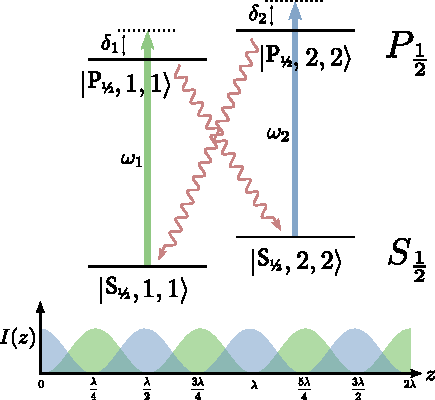
\includegraphics[width=0.65\textwidth]{figures/unsorted/cooling_simplified.pdf}
\caption{\label{fig:cooling_simplified}An idealised depiction of the cooling scheme, with repump lasers and undesired states not shown. Two lasers on the D$_1$ line are used for cooling, both linearly polarised, and arranged so as to form two interleaved standing waves. Both are blue detuned from the transitions they target, and they differ by about $6.8\,$GHz. This difference means that the alignment of the two standing waves can only be maintained over a distance of about a centimetre.}
\end{center}
\end{figure}

The scheme involves four lasers, two for cooling and two for repumping. First let's focus on the cooling lasers only. Looking at Figure \ref{fig:cooling_simplified}, imagine that we have a rubidium atom at $z=0$ and in the $|1,1\rangle$ hyperfine groundstate. Here our atom sees no light, as the intensity of the cooling laser labeled $\omega_1$ is zero, and it is in the wrong state to be pumped by the $\omega_2$ laser (which is not resonant with any transitions from the $|1,1\rangle$ groundstate).

As our atom moves rightward however, it will have to climb the repulsive potential hill formed by the $\omega_1$ laser. As it does so, its $|1,1\rangle$ excited state probability will increase, and along with it, the probability of spontaneous emission. Spontaneous emission will be most likely to occur near the top of the potential hill where the laser intensity---and hence the excited state probability---is greatest.

The most likely groundstate for the atoms to decay to from the $|1,1\rangle$ excited state is the $|2,2\rangle$ groundstate, and this is most likely to occur near $z=\frac\lambda4$. If this occurs, we now have an atom in the $|2,2\rangle$ groundstate at $z=\frac\lambda4$, a situation similar to that in which it started. Again, out atom now sees no light, but which laser has zero intensity and which targets the wrong transition are swapped.

As our atom continues rightward, it now has to contend with the potential hill formed by the $\omega_2$ laser, and is most likely to undergo spontaneous emission from the $|2,2\rangle$ excited state near the top of the potential hill. This time emission is most likely to put the atom into the $|1,1\rangle$ groundstate.

This process repeats, with atoms repeatedly climbing potential hills and being cooled. They spend approximately half their time in the $|1,1\rangle$ groundstate, allowing us to take advantage of the strong interspecies repulsion that that state entails for our two atomic species.

Of course, as is always the case, things aren't that simple. Whilst the two spontaneous decays mentioned above are the most likely, they are by no means the only possibilities. Some spontaneous decays will put the atoms back into the groundstate from which they came, with no harm done except a little extra heating from the photon recoil. Other decays however will put our atom into states that are not involved in the cooling scheme, where they will remain with no further cooling unless we do something about it. For this we need repump lasers (Figure \ref{fig:cooling_full}).

There are three states that the atom might end up in as a result of decay from the two excited states involved in the cooling process, and two repump lasers are used to excite them to three $P_\frac32$ states. Two of these transitions are similar enough that they can be addressed with the same laser.

\begin{figure}
\begin{center}
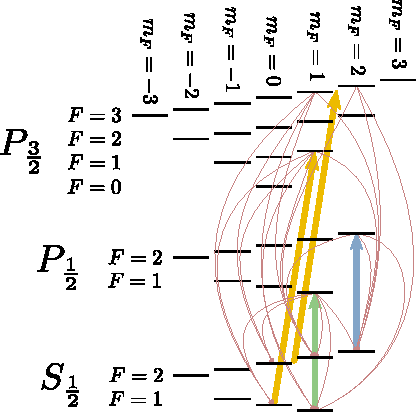
\includegraphics[width=0.65\textwidth]{figures/unsorted/cooling_full.pdf}
\caption{\label{fig:cooling_full} The full cooling scheme, including repump lasers (yellow), cooling lasers (blue and green), and all possible decay paths (red). The repump beam which is drawn in between two ground and excited states has a frequency equal to the average of those two transitions. }
\end{center}
\end{figure}

\subsection{Methods}

This scheme was simulated for the case of a single atom, with the internal state of the atom modelled with the Schr\"odinger equation in the spin basis, the state vector being a complex 32-vector\footnote{One complex number for each state in Fig. \ref{fig:cooling_full}.}. The coupling terms between each pair of states were computed by solving the eigenvalue problem in the spin basis, with the Hamiltonian including Zeeman terms, and projecting the resulting eigenvectors onto the zero field eigenvectors. The zero field eigenvectors have easily computed coupling constants\footnote{Using the dipole approximation and the rotating wave approximation, following the derivation in \cite[p 9]{steck_rubidium_2010}.}, a weighted sum of which gives the coupling constants for the states at higher field\footnote{Each energy eigenstate at nonzero field is a superposition of exactly two of the zero field eigenstates.}. Since the coupling constants are dependent on the laser intensity, they were re-computed constantly as the atom moved through different intensities of the cooling beams. This process produced a set of 32 coupled differential equations for the complex amplitudes of each state \cite[p 4]{metcalf_laser_1999}, of the form :

\begin{equation}
i\hbar\frac{dc_e(t)}{dt} = -\frac12e\sum_{g,\ n} E_n \langle g |  q_n | e \rangle c_g(t) \ee^{-\ii\delta_{nge}t},
\end{equation}
and
\begin{equation}
i\hbar\frac{dc_g(t)}{dt} = -\frac12e\sum_{e,\ n} E_n \langle g |  q_n | e \rangle c_e(t) \ee^{\ii\delta_{nge}t},
\end{equation}
where each $c(t)$ is the complex amplitude of one state; the $e$ indices are over the excited states and the $g$ indices over the groundstates\footnote{not to be confused with the electron charge or base of the natural logarithm, also used but not as indices.}; the $n$ indices are over the lasers, with $E_n$ being the amplitude of the $n$\textsuperscript{th} laser's electric field, $\delta_{nge}$ the detuning of the $n$\textsuperscript{th} laser from the transition between the $g$\textsuperscript{th} ground and $e$\textsuperscript{th} excited states, and $\langle g |  q_n | e \rangle$ the dipole moment between the $g$\textsuperscript{th} ground and $e$\textsuperscript{th} excited states for the polarisation of the $n$\textsuperscript{th} laser.

The external motion of the atom was modelled classically, with the atom having a definite position and velocity in one dimension. The force on the atom was computed using the gradient of the light shift that the two groundstates experience due to the standing waves formed by the cooling beams \cite[eqn 3.16, p 33]{metcalf_laser_1999}. The atom's state was projected onto the two groundstates which see the cooling lasers. The resulting force on the atom was used in the classical equation of motion.

Spontaneous emission was handled by at each integration timestep, summing up all the population in $P_\frac12$ and $P_\frac32$ excited states, weighted by their decay rates (equal to the natural linewidth). This gave the probability of decay per unit time. Multiplying by the duration of one timestep, and comparing with a random number then determined whether a decay was to occur.

In the event of a decay, one excited state was randomly chosen, weighted by their populations, and then one groundstate, weighted by the transition strengths from the excited state. All population was then put into that groundstate and the simulation continued, with one photon's worth of momentum in a random direction added to the atom's external state to account for photon recoil.

The equations of motion were solved using fourth order Runge--Kutta integration, with the error monitored by verifying that the overall probability summed over all states remained close to unity.

\subsection{Results}

\begin{table}
    \renewcommand{\arraystretch}{2.0}
    \makebox[\textwidth][c]{
    \begin{tabular}{|c|p{3.5cm}|r|r|c|}\hline
    Type & Transition(s) targeted & Detuning & Intensity (per beam) & Polarisation\\\hline
    cooling (standing wave) & $|S_\frac12,2,2\rangle\rightarrow |P_\frac12,2,2\rangle$ & + $66.6\,$MHz & $5.0\,$mW$\,$cm$^{-2}$ & $\pi$ \\
    cooling (standing wave) & $|S_\frac12,1,1\rangle\rightarrow |P_\frac12,1,1\rangle$ & + $31.9\,$MHz & $5.0\,$mW$\,$cm$^{-2}$ & $\pi$ \\
    repump (single beam) & \parbox{5cm}{\ \\ $|S_\frac12,2,1\rangle\rightarrow |P_\frac32,2,2\rangle$ \\
                           $|S_\frac12,2,0\rangle\rightarrow |P_\frac32,2,1\rangle$} & Midway between & $50.0\,$mW$\,$cm$^{-2}$ & $\sigma^+$ \\
    repump (single beam) & $|S_\frac12,1,0\rangle\rightarrow |P_\frac32,1,1\rangle$  & $0$ & $10.0\,$mW$\,$cm$^{-2}$ & $\sigma^+$ \\

    \hline
    \end{tabular}
    }
    \caption{The parameters used in the laser cooling simulations. There are four lasers, each with a specified polarisation, intensity, and detuning from the transition it targets.}\label{table:numbers}
\end{table}

The laser parameters used in the simulation are shown in Table \ref{table:numbers}. The magnetic field strength used was 34$\,$G.

The simulation was run for 715 million integration timesteps of 20 picoseconds each\footnote{Which is about ten timesteps per oscillation of the fastest oscillating terms, which oscillate at a rate equal to approximately half the 6.8GHz hyperfine splitting of the rubidium groundstates.}, for a total of 14.3 milliseconds of simulation time. This took 14 days of computer time. In that time, the atom moved a maximum distance of 26 micrometres from its starting position, and its final position was 790 nanometres from its starting position. The atom's initial velocity was 195 millimetres per second, and during the simulation it reversed the direction of its velocity 2226 times. 4103 photons were emitted, for an average scattering rate of 2.87$\times$10$^\up{5}$ photons per second.

Computing the time averaged energy of the atom over the whole simulation using:
\begin{equation}
\langle E \rangle = \frac12 m_\up{Rb} \langle v^2 \rangle,
\end{equation}
and converting to temperature units with $k_B T = \langle E \rangle$ gives a temperature of $8.1\,\upmu$K. Since this is only a one-dimensional simulation, a temperature approximately three times higher would be expected in three dimensions, as the atom would have approximately the same amount of energy in each spatial degree of freedom.

A histogram of what fraction of the time the atom spent at different velocities is show in Figure \ref{fig:cold_atom}.

\begin{figure}
\begin{center}
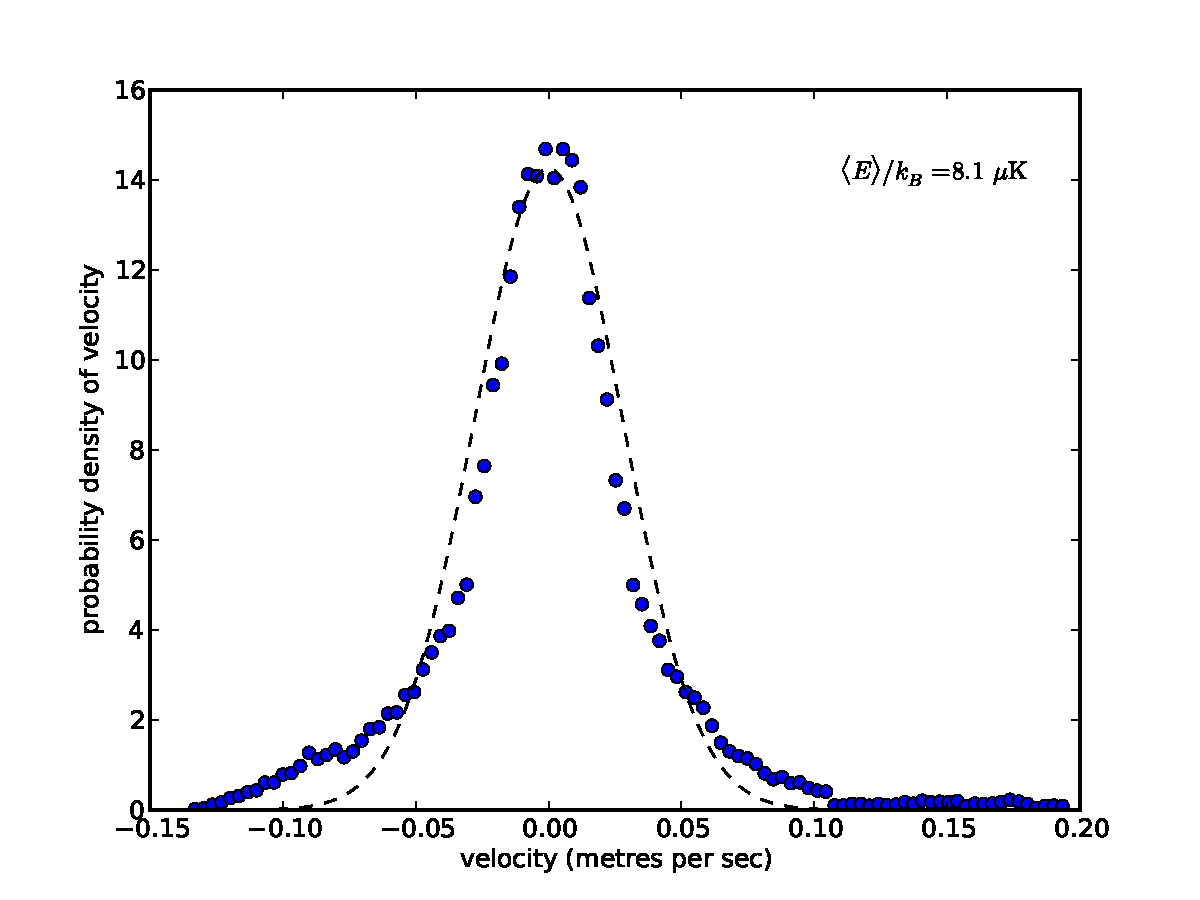
\includegraphics[width=\textwidth]{figures/unsorted/cold_atom.pdf}
\caption{\label{fig:cold_atom} Histogram of atom velocity over time, normalised such that it can be interpreted as a probability density. A best-fit Maxwell-Boltzmann distribution is shown as the dotted line. It is no surprise that it is not a good fit---there is no thermalisation happening since we have only one atom and no collisions. The average energy is more informative than the fit parameters for determining the temperature that an ensemble of such atoms would have if they were allowed to thermalise. This is because the average energy would stay constant throughout thermalisation, whereas the fit parameters would not. Only for a fully thermal distribution would the two methods agree. The long tail visible to the right is the atom's initial slowdown from its starting velocity.}
\end{center}
\end{figure}

This one-dimensional temperature corresponds to approximately 44 recoil energies, and if extrapolated to three dimensions, about 132 recoils. Given that the potassium vortex potentials are at most about 15 recoils deep without a Feshbach resonance, and only about 8 recoils when you consider that the rubidium is not in the ideal state half of the time, this result will only be able to keep rubidium atoms trapped in vortex cores if we can get a factor of 20 or so increase in the interspecies repulsion via a Feshbach resonance.

This simulation has not, however, been optimised. Whilst some parameters were computed from others based on assumptions about optimal scattering rates and the like, no attempt has been made to scan over parameter space to see if the temperature can be made lower. I plan on using a genetic algorithm to optimise the parameters by managing a population of simulations running on one of the university clusters. A significant speed up should be possible by excluding from the simulation the atomic states that were shown in the first run never to become occupied. This will eliminate approximately two thirds of the states, and since the simulation is quadratic in the number of states, this should provide an approximately $10\times$ increase in simulation speed.

The simulation will also require repetition to verify that the results still hold when a significant error, recently discovered, is corrected. The error is that the Zeeman sublevels used in the simulation were all incorrect by a sign. There is a large degree of symmetry with this change, and the scattering rates between all involved states are almost identical, so I am confident that this will only slightly change the results.

Ultimately only experimentation will show whether this method is viable, and what the optimal parameters are, but since it requires a large number of lasers, it is likely worth further theoretical investigation before attempting to implement it.

\subsection{Vortex-assisted Sisyphus cooling}\label{sec:vortexcooling}

[COMMENT ON HIDDEN VARIABLES - PRESENTED HERE TO MAKE A POINT]

Another idea for a cooling scheme is to use the vortex potential itself as a spatial discriminator for transferring atoms between states. Similar to how a \mot\ traps atoms by bringing them into resonance with optical pumping only when they are some distance from the trap's centre, we could use the shape of the vortex potential to bring an \rf\ or microwave transition into resonance only when trapped tracer particles are some way up the side of a vortex core.

\begin{figure}
\begin{center}
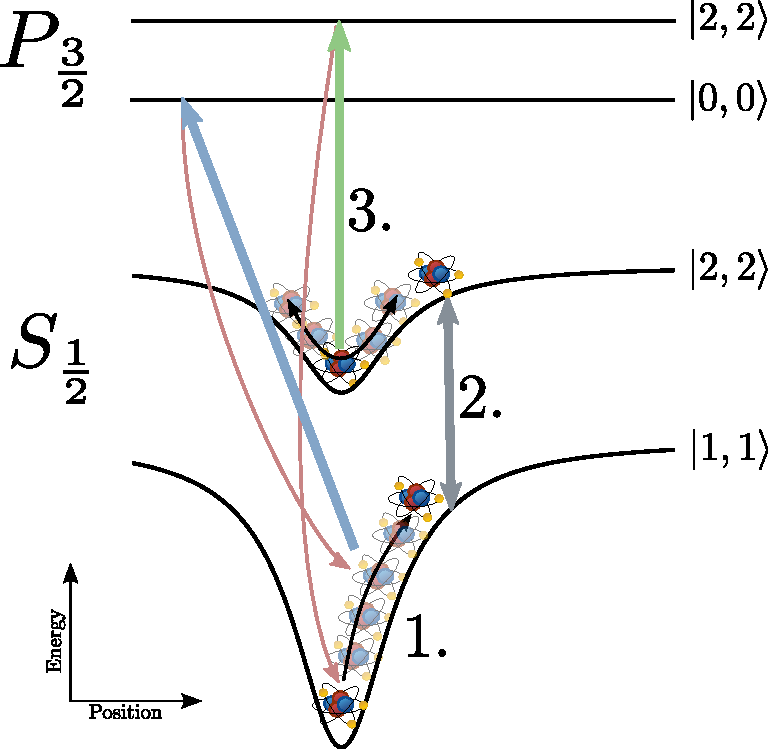
\includegraphics[width=0.7\textwidth]{figures/unsorted/vortexcooling.pdf}
\caption{A basic description of the vortex-assisted cooling scheme.
\protect\\
1. The rubidium atom in its $|1,1\rangle$ groundstate repeatedly scatters photons from the laser marked with the blue arrow, climbing the vortex potential as it does so. The optical transition's linewidth is large enough that the energy shift due to the vortex potential does not move it off resonance.
\protect\\
 2. An \rf\ or microwave transition however, has an extremely narrow linewidth; its effective linewidth is dependent only on the \rf/microwave power. A microwave transition (grey arrow) comes into resonance only when the atom moves sufficiently far from the vortex core's centre, and coherently transfers population into the $|2,2\rangle$ groundstate.
 \protect\\
 3. The atom oscillates back and forth in the much shallower vortex potential that its $|2,2\rangle$ groundstate experiences. It is pumped weakly by the laser marked with the green arrow, and after a random time delay (and hence at a random position) spontaneously decays back to the $|1,1\rangle$ groundstate.
}\label{fig:vortexcooling}
\end{center}
\end{figure}

The basic idea is outlined in Figure~\ref{fig:vortexcooling}. In the presence of the Feshbach resonance, atoms in the $|1,1\rangle$ state will scatter some tens of photons, using whichever transition is most likely to have them decay to the same groundstate with minimal repumping (transitioning to the $|0,0\rangle$ excited state on the $D_2$ line looks to be the best choice). As the atom scatters photons, it climbs the side of the vortex potential, converting its new found kinetic energy (from photon recoil) into potential energy.

Due to the state-dependence of the interspecies scattering length, the vortex potentials for different states have different depths. This means that the \rf\ or microwave frequency required to transition between the different hyperfine states and Zeeman sublevels varies as a function of space, and can be tuned so as to only be resonant with atoms which have nearly escaped the vortex core.

The atom is then transferred into a different hyperfine or Zeeman state (the $|2,2\rangle$ groundstate should suit) and the hope is that it then lacks the kinetic energy to escape the (shallower) vortex potential it now finds itself in. Rather, it will oscillate back and forth in the well until a weak laser pumps it back into the $|1,1\rangle$ groundstate via spontaneous emission from some excited state (again chosen to maximise the decay probability to $|1,1\rangle$; the $|2,2\rangle$ $P_\frac32$ excited state looks to be a good choice.)

If this goes to plan, statistically the atom will be closer to the center of the  $|1,1\rangle$ vortex potential than when it left. Provided its corresponding drop in potential energy makes up for all the photon scattering (which provides fluorescence imaging), then we have a cooling scheme. It is yet another Sisyphus effect, with the atom climbing steep vortex potential hills and descending shallower ones.

This scheme will be simulated to determine its viability; preliminary calculations haven't turned up any problems yet.

% Paths: bilbo.tk: ~/laptop_backup/Desktop/current_work/sympathetic_cooling/
%                  ~/oldserver/bilbo/particle_tracking_higher_scattering_length
%                  ~/laptop_backup/Desktop/current_work/paper%20simulations/
%                  ~/laptop_backup/Desktop/current_work/paper
%                  ~/laptop_backup/Desktop/current_work/DPGPoster
% Compare to honours thesis - don't include stuff already in honours thesis!

